\newcommand\BackgroundPic{
\put(0,0){%
\parbox[b][\paperheight]{\paperwidth}{%
\vfill%
\centering%

\includegraphics[width=\paperwidth,height=\paperheight,keepaspectratio]{cover0.jpg}%
\vfill%
}}}\AddToShipoutPicture*{\BackgroundPic}%
\AddToShipoutPicture*{\put(0,0){%
\parbox[b][\paperheight]{\paperwidth}{%
\definecolor{gold}{rgb}{0.77,0.69,0.37}%
\vfilneg\centering\color{white}%
\vskip 3cm\resizebox{.95\stockwidth}{!}{\textls[100]{HARRY POTTER AND THE}}%
\vskip 2mm%
\color{gold}%
\newlength{\rationalh}\settoheight{\rationalh}{%
\resizebox{.95\stockwidth}{!}{\textls[20]{RATIONALITY}}}
\resizebox{!}{\rationalh}{\textls[50]{METHODS}}%
\hfil\resizebox{!}{\rationalh}{\textls[50]{OF}}%
\vskip 2mm%
\resizebox{.95\stockwidth}{!}{\textls[20]{RATIONALITY}}%
\vskip 8mm%
\color{white}%
\resizebox{.5\stockwidth}{!}{\textls[50]{\scshape{}by Eliezer Yudkowsky}}
\vfil
\resizebox{.5\stockwidth}{!}{\textls[50]{\scshape chapters 1--\ref{last:chapter} plus omake files}}%
\color{black}
\vskip 1cm\ %\vfil%
}}}%
\ %
%~ \cleartorecto
%~ \vspace{4cm}
%~ \begin{center}
%~ 
%~ \hp
%~ 
%~ \vspace*{2.5cm}
%~ 
%~ \huge\MakeUppercase{Harry James Potter-Evans-Verres}
%~ 
%~ \vspace*{0.5cm}
%~ 
%~ \Large\MakeUppercase{and the Methods of Rationality}
%~ 
%~ \vspace{6cm}
%~ \Large Chapters 1 to \ref{last:chapter}
%~ \end{center}
%~ \thispagestyle{empty}
\clearpage
\begin{center}
\vspace*{2cm}

\thispagestyle{empty}
Based on the characters of

\vspace*{.5cm}

\Large J. K. ROWLING \normalsize 

\vspace*{.5cm}

and her books:

\vspace*{.5cm}

{
	\newcounter{books_list_counter}
	\def \hpBook #1{  
		\addtocounter{books_list_counter}{1} 
		\textit{Harry Potter and the #1} \par
		Year \numtoName{\value{books_list_counter}} at Hogwarts
		\smallskip\par
	}
	
	\hpBook{Sorcerer’s Stone}
	\hpBook{Chamber of Secrets}
	\hpBook{Prisoner of Azkaban}
	\hpBook{Goblet of Fire}
	\hpBook{Order of the Phoenix}
	\hpBook{Half-Blood Prince}
	\hpBook{Deathly Hallows}
}
\end{center}

\clearpage

\begin{center}
\thispagestyle{empty}
{\hp
\Huge\MakeUppercase{Harry Potter}\vspace*{0.5cm}

\Large\MakeUppercase{and the Methods of Rationality} %\vspace*{1cm}
 
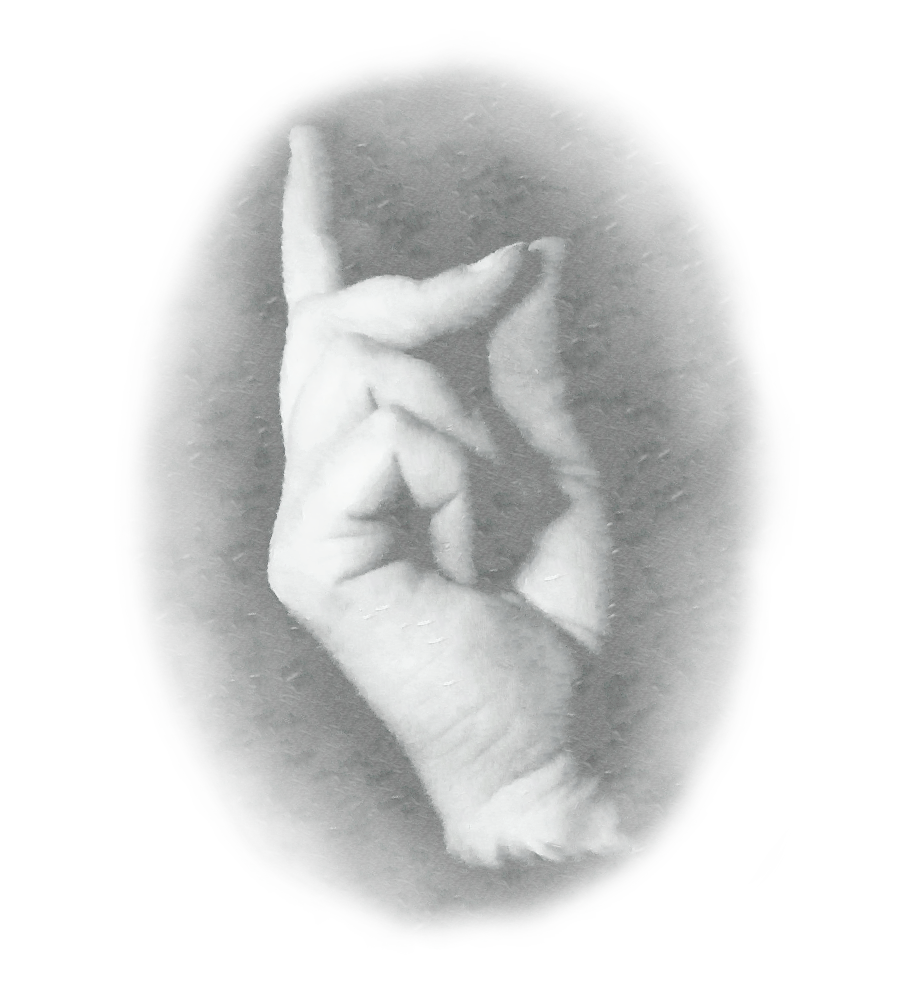
\includegraphics[scale=0.5]{bubble0.png} 

\Large BY \vspace*{.25cm}

\huge ELIEZER YUDKOWSKY%\vspace*{1cm}

\normalsize
Formatted by some random fans of a fan
}

\vspace{3cm}
Find the original text (perhaps with added chapters) at:\\
\url{http://hpmor.com} \\
% or \\
% \url{http://www.fanfiction.net/s/5782108}
%/1/Harry\_Potter\_and\_the\_Methods\_of\_Rationality

\end{center}
\clearpage

%~ \chapter*{Reader Advisory}
%~ \thispagestyle{empty}
%~ Please note that, despite being Harry Potter fan-fiction, this is a \emph{grown-up book}. That does \emph{not} mean that it is only for grown-ups, nor that all grown-ups can or should read it; it is the book itself that is grown up. Some parts of the story might have potentially traumatic associations for some readers. Not all the characters are nice people, and some of their actions, thoughts or words can be unsettling. (Actually, that’s an understatment; they often are.)
%~ 
%~ They’re also bewildering, heartwarming and, more often than not, awesome. A completely non-scientific study of reades revealed that side-effects include wide-eyed awe, uncontrolable fits of laughter, giggling, and falling from seats, and sometimes urges to consume a certain green beverage. By the way, readers drinking or eating while reading are advised to keep a towel nearby. 
%~ 
%~ Readers with a more delicate constitution should check \begin{center}\url{http://wiki.lesswrong.com/wiki/Methods\_Of\_Rationality\_(fanfiction)/Trigger\_warnings}\end{center} for more specific warnings, or ask a friend to read the story before them.
